\documentclass[11pt]{article}

% Packages
\usepackage[margin=1in]{geometry}
\usepackage{amsmath,amssymb,amsfonts}
\usepackage{graphicx}
\usepackage{booktabs}
\usepackage{hyperref}
\usepackage{natbib}
\usepackage{caption}
\usepackage{subcaption}
\usepackage{xcolor}

\hypersetup{colorlinks=true, linkcolor=blue!60!black, citecolor=green!50!black, urlcolor=blue!70!black}

\newcommand{\bpb}{\text{BPB}}
\newcommand{\E}{\mathbb{E}}

\title{Partition Function Inflation in Hashed N-Gram Caches:\\Why Unnormalized Scoring Functions Appear to Improve\\Neural Language Model Compression}
\author{Robert Sneiderman\thanks{Correspondence: \texttt{RobbySneiderman@gmail.com}. Code and data: \url{https://github.com/Robby955/partition-function-inflation}.}}
\date{April 2026}

\begin{document}
\maketitle

% ====================================================================
\begin{abstract}
Hash-table n-gram caches report large bits-per-byte (BPB) improvements over neural baselines in transductive compression benchmarks, with smaller hash tables (more collisions) consistently producing lower unnormalized scores than larger ones. We show that these gains are largely an artifact of partition function inflation in the unnormalized scoring function. Under a uniform-hashing collision model, the partition function $Z$ satisfies an exact recurrence whose mean-field fixed point is $Z^* \approx (n_c + VL)/(n_c + L)$, exceeding 1,000 for typical settings ($V{=}1024$, load factor $L{\approx}59$). Empirical measurement of $Z$ at four bucket sizes is consistent with the recurrence. A partial normalization sweep ($\lambda \in [0, 1]$, dividing by $Z^\lambda$) shows BPB increasing linearly with $\lambda$ (as expected from the additive log-score structure), crossing the 1.13 neural baseline at $\lambda \approx 0.25$. A rate-matched random collision control replicates 99.4\% of the observed BPB gap in this configuration across 8 independent remap seeds ($\text{std} = 0.00004$ BPB), indicating count inflation rather than distributional smoothing as the primary driver. An independent collision-free trie baseline (PR~\#511, different architecture) achieves only $-0.0013$ BPB improvement---${\sim}775\times$ smaller than the 0.975-point unnormalized hash-based apparent gain. These results hold across three model seeds, with negligible variance relative to effect sizes, and are consistent with the late March 2026 closure of dozens of cache-augmented benchmark submissions.
\end{abstract}

% ====================================================================
\section{Introduction}

Cache-augmented neural language models dominated the OpenAI Parameter Golf challenge, which evaluates bits-per-byte compression of FineWeb validation data under a 16\,MB artifact and 10-minute compute constraint. Hashed n-gram caches combined with neural transformer predictions reported BPB scores as low as 0.083 (PR~\#986), a ${\approx}$93\% reduction from the neural-only baseline of 1.13 BPB. By late March 2026, dozens of submissions incorporated some form of hashed n-gram caching with recursive Dirichlet smoothing.

Smaller hash tables---which produce more hash collisions---consistently outperformed larger ones. At a fixed Dirichlet concentration parameter $\alpha = 2$, a 1M-bucket table ($2^{20}$ buckets, load factor $L \approx 59$) scored 0.155 BPB while a 64M-bucket table ($2^{26}$, $L \approx 0.92$) scored 1.774 BPB. This ordering held across all nine concentration values tested and across six distinct per-order concentration profiles. Hash collisions, conventionally treated as approximation error, appeared to help.

Submission structure suggests the cache dominated the reported score: PR~\#913 used a ${\sim}$500K-parameter model (vs.\ 27M standard) yet achieved 0.089 BPB, though this does not prove the neural component was negligible---only that a tiny model plus cache sufficed under the unnormalized metric.

In late March 2026, competition organizers closed dozens of n-gram cache submissions after community analysis revealed that these systems did not compute properly normalized probability distributions. The scoring function evaluated only the true token's recursive score $p_K(t)$ (Eq.~\ref{eq:recursion}), without verifying that the partition function $Z = \sum_t p_K(t)$ equals 1. Independent confirmation came from PR~\#978 (AnirudhRahul), whose attempt to normalize the cache distribution yielded 1.51 BPB---far above the originally reported score. This paper gives a quantitative diagnosis of why this omission produces the observed ranking and apparent gains.

\paragraph{Contributions.}
\begin{enumerate}
\item We derive an exact recurrence for the partition function $Z$ of a recursive Dirichlet-multinomial cache: $Z_n = (S^{(n)} + \alpha Z_{n-1})/(c^{(n)} + \alpha)$. Under a uniform-hashing mean-field collision model, the approximate fixed point is $Z^* \approx (n_c + VL)/(n_c + L)$, with contraction rate $\gamma = \alpha/(c + \alpha)$. A heuristic constant-$\gamma$ approximation yields a closed-form solution; the exact variable-coefficient version appears in the appendix. For singleton contexts at standard settings, $Z^*$ exceeds 1,000 and the recurrence converges in 2--3 cache steps (Section~\ref{sec:theory}).

\item We demonstrate through a 36-configuration controlled sweep that the $Z$ recurrence is consistent with the observed bucket-count ranking and helps organize the main concentration trends (Section~\ref{sec:experiments}).

\item A rate-matched random collision control demonstrates that count-inflation magnitude, not collision-partner structure, accounts for nearly all of the effect in the tested configuration: across 8 independent remap seeds, random collisions replicate 99.4\% of the observed BPB gap with near-zero variance ($\text{std} = 0.00004$ BPB) (Section~\ref{sec:experiments}).

\item Under post-hoc normalization ($\lambda = 1$, directly measured at 4.10 BPB at 1M), all four tested bucket-size configurations produce BPB far worse than the neural baseline; step-wise renormalization (4.15 BPB at 1M) gives a comparable outcome. A partial normalization sweep ($\lambda \in [0,1]$, dividing by $Z^\lambda$) crosses the neural baseline at $\lambda \approx 0.25$ with a measured slope of 3.94 BPB per unit $\lambda$, consistent with Eq.~\ref{eq:lambda} (Section~\ref{sec:consequences}).

\item The Pitman-Yor discount parameter $d$ degrades performance, consistent with the $Z$ mechanism: discounting reduces count mass $S$, shrinking $Z$ and therefore the unnormalized score advantage. The optimal concentration is approximately stable across high-load-factor configurations (Section~\ref{sec:consequences}).
\end{enumerate}

% ====================================================================
\section{Partition Function Analysis}
\label{sec:theory}

\subsection{Setup}

We study a transductive compression system combining a 27M-parameter GPT-style transformer with a hashed recursive n-gram cache. The system operates on BPE-1024 tokens (vocabulary size $V = 1024$) and evaluates on 62M tokens of FineWeb validation data.

\paragraph{Hash table structure.} For each n-gram order $k \in \{2, 3, \ldots, 7\}$, the system maintains two hash tables of $B$ buckets each: a \emph{context table} storing how often each context prefix has been seen, and a \emph{full table} storing how often each (context, target) pair has been seen. Both tables use XOR-prime hashing:
\[
h(t_1, \ldots, t_k) = (t_1 \cdot p_1) \oplus (t_2 \cdot p_2) \oplus \cdots \oplus (t_k \cdot p_k) \bmod B
\]
where $p_i$ are fixed primes and $\oplus$ denotes bitwise XOR. Multiple distinct n-grams may hash to the same bucket. Each of the 6 n-gram orders maintains its own independent pair of hash tables. The load factor $L = N/B$, where $N$ is the number of tokens evaluated (i.e., the number of per-order insertions, equal to the evaluation sequence length; see Table~\ref{tab:exp1}), characterizes the expected number of entries per bucket.

\paragraph{Recursive Dirichlet-multinomial mixing.} Given a context, the system computes a predictive distribution for the next token $t_j$ by recursive backoff from the neural prior $\pi(t)$ through ascending n-gram orders:
\begin{align}
p_1(t) &= \pi(t) \label{eq:base} \\
p_n(t) &= \frac{\tilde{f}_t^{(n)} + \alpha_n \cdot p_{n-1}(t)}{c^{(n)} + \alpha_n} \qquad \text{for } n = 2, \ldots, K \label{eq:recursion}
\end{align}
where $K$ is the highest n-gram order ($K = 7$ in our experiments, giving $K - 1 = 6$ recursive cache steps), $\tilde{f}_t^{(n)} = \min(f_t^{(n)},\, c^{(n)})$ is the clamped hashed count of the full n-gram at order $n$, $c^{(n)}$ is the hashed context count, and $\alpha_n$ is the concentration parameter. We write $c^{(n)}$ for the general per-order notation, $c_{\text{obs}}$ when emphasizing the collision-inflated nature of the count ($c_{\text{obs}} = n_c + L$), and abbreviate to $c$ where the meaning is clear from context. The clamp prevents any single token's count from exceeding the context total; in the high-load regime ($L \geq 4$) clamp activations are negligible because $f_t \approx L < c_{\text{obs}} \approx n_c + L$, and do not materially affect $Z$. All experiments, including $Z$ measurements, use the clamped form. This recursion is algebraically equivalent to interpolated backoff with weight $\lambda_n = c^{(n)}/(c^{(n)} + \alpha_n)$, though $\tilde{f}_t/c$ is not a proper distribution when $\sum_t \tilde{f}_t \neq c$ due to collisions.

\paragraph{The scoring function.} In the competition implementation, BPB is computed as:
\[
\bpb_{\text{unnorm}} = -\frac{1}{N_{\text{bytes}}} \sum_j \log_2 p_K(t_j)
\]
where the sum runs over all evaluation positions $j$. The partition function $Z_j = \sum_t p_K(t)$ is never computed. If $Z \neq 1$, the reported BPB is not a valid compression rate.

\subsection{The partition function recurrence}

We derive the partition function $Z_n = \sum_t p_n(t)$ at each recursive level.

\paragraph{Base case.} The neural prior is properly normalized: $Z_1 = \sum_t p_1(t) = 1$.

\paragraph{Recursive step.} At order $n$:
\begin{equation}
Z_n = \sum_t p_n(t) = \frac{\sum_t \tilde{f}_t^{(n)} + \alpha_n \cdot Z_{n-1}}{c^{(n)} + \alpha_n} = \frac{S^{(n)} + \alpha_n \cdot Z_{n-1}}{c^{(n)} + \alpha_n}
\label{eq:z_recurrence}
\end{equation}
where $S^{(n)} = \sum_t \tilde{f}_t^{(n)}$ is the sum of clamped full-table counts across all $V$ tokens. (The mean-field analysis below uses unclamped counts $f_t^{(n)}$ for tractability. Since $\tilde{f}_t \leq f_t$, clamping can only reduce $S$ and therefore $Z$; the unclamped fixed point~\eqref{eq:z_star} is an upper bound on the clamped system's $Z$. Empirically, clamp activations are rare in the high-load regime ($L \geq 4$): at 1M buckets, fewer than 0.3\% of token lookups trigger the clamp, and the effect on the trajectory-averaged $Z$ is negligible.)

The following three properties hold exactly for the implemented recursion (Eq.~\ref{eq:recursion}), without any approximation:

\smallskip
\noindent\textbf{Fact 1} (Z recurrence). \emph{$Z_n = (S^{(n)} + \alpha_n Z_{n-1})/(c^{(n)} + \alpha_n)$ follows by summing Eq.~\ref{eq:recursion} over $t$.}

\smallskip
\noindent\textbf{Fact 2} (Collision-free normalization). \emph{If counts are exact (no collisions), then $S^{(n)} = c^{(n)}$ and $Z_n = 1$ for all $n$ by induction from $Z_1 = 1$. With hash collisions, $S^{(n)} > c^{(n)}$ generically, so $Z_n > 1$.}

\smallskip
\noindent\textbf{Observation 3} (Empirical vocabulary ceiling). \emph{In all measurements, $Z_n \leq V$. If $S^{(n)} \leq V \cdot c^{(n)}$ at every order (i.e., no single token's bucket count exceeds the full context count), then induction from $Z_1 = 1$ gives $Z_n \leq V$. This condition holds in all our experiments; we have not verified it analytically for all hashing regimes. At 1M buckets, the observed maximum is $Z_{\max} = 1023.96 \approx V$, consistent with the fixed-point formula saturating at $V$.}

\smallskip

\paragraph{Collision model (mean-field approximation).} Each token $t$ is looked up in a separate full-table bucket via $\text{hash}(\text{context}, t)$. Under the assumption of approximately uniform hashing---supported by the alt-hash test in Section~\ref{sec:experiments}, where two independent prime sets produce similar results (gap = 0.007 BPB)---with $N$ total insertions and $B$ buckets, each bucket accumulates approximately $L = N/B$ entries on average:
\begin{align}
\E[f_t^{(n)}] &= k_t + L \\
\E[S^{(n)}] &= n_c + V \cdot L
\end{align}
where $k_t$ is the true count of (context, $t$) and $n_c = \sum_t k_t$ is the true (collision-free) context count. The observed context count is $c_{\text{obs}} = n_c + L$. (The expectations above use unclamped $f_t$. Note that $\E[\min(f_t, c)] \leq \E[f_t]$, so the unclamped formula~\eqref{eq:z_star} provides an upper bound on the clamped system's fixed point. The bound is tight when clamp activations are rare---empirically the case at $L \geq 4$, where bucket counts $f_t$ are concentrated near $L \ll c_{\text{obs}}$. At low load factors or in tail events, the clamp may materially reduce $Z$ below the unclamped prediction.)

\paragraph{Fixed point (mean-field).} Substituting expected values for $S$ and $c_{\text{obs}}$ (a mean-field approximation, since $\E[S/c] \neq \E[S]/\E[c]$ in general) and setting $Z_n = Z_{n-1} = Z^*$ in~\eqref{eq:z_recurrence}:
\begin{equation}
Z^* \approx \frac{\E[S]}{\E[c_{\text{obs}}]} = \frac{n_c + V \cdot L}{n_c + L}
\label{eq:z_star}
\end{equation}

Empirically, the induced error in $\log_2 Z$ is small: across 8 independent remap seeds the BPB varies by only $\text{std} = 0.00004$, and the singleton formula overestimates the trajectory-averaged $\E[\log_2 Z]$ by at most 4\% at high load (Section~\ref{sec:scaling}), consistent with tight concentration of $S/c_{\text{obs}}$ at the load factors tested. Notably, $Z^* > 1$ for any $L > 0$ and $V > 1$, with $Z^* \to V$ as $L \to \infty$, so partition function inflation is unavoidable under unnormalized scoring whenever hash collisions are present. The fixed point satisfies $1 < Z^* \leq V$, with $Z^* \to 1$ as $L \to 0$. For singleton contexts ($n_c = 1$) at 1M buckets ($B = 2^{20}$, $L \approx 59$): $Z^* = (1 + 1024 \times 59)/(1 + 59) \approx 1{,}007$. At 64M buckets ($B = 2^{26}$, $L \approx 0.92$): $Z^* = (1 + 1024 \times 0.92)/1.92 \approx 492$. For frequently observed contexts ($n_c \gg 1$), $Z^*$ is lower because real counts dominate over collision noise. The singleton case provides an upper bound.

\paragraph{Stability of the mean-field ratio.} The mean-field step replaces $S/c_{\text{obs}}$ with $\E[S]/\E[c_{\text{obs}}]$. Under uniform hashing, the $V$ full-table bucket counts are sums of approximately $L$ entries each, with weak dependence introduced by the deterministic hash function (all $V$ lookups at one position share the same context hash). Rather than claim formal independence, we note that the ratio $S/c$ is empirically stable: across 8 independent remap seeds (Section~\ref{sec:experiments}), the BPB varies by only $\text{std} = 0.00004$, confirming that the mean-field proxy $\E[S]/\E[c]$ is tight in practice. The deterministic hash dependence among token lookups does not substantially affect the realized ratio at the load factors tested.

\subsection{Closed-form solution}

The recurrence~\eqref{eq:z_recurrence} is an affine map in $Z_{n-1}$. With the propagation weight $\gamma_n = \alpha_n/(c^{(n)} + \alpha_n)$, starting from $Z_1 = 1$ (normalized neural prior), applying $K - 1$ cache steps, and approximating $\gamma_n \approx \gamma$ as constant across orders:
\begin{equation}
Z_K \approx Z^* - (Z^* - 1) \cdot \gamma^{K-1}
\label{eq:closed_form}
\end{equation}

This is a heuristic approximation: it assumes both $\gamma_n$ and the affine offset $A_n = S^{(n)}/(c^{(n)} + \alpha_n)$ are roughly constant across orders. In practice, $\gamma_n$ varies little because $c^{(n)}$ dominates $\alpha_n$ at all orders where context counts are substantial. At 1M buckets with $\alpha = 2$: $\gamma = 2/62 \approx 0.032$. After two cache steps, $Z$ is within 0.1\% of its fixed point. At 64M buckets: $\gamma = 2/3.92 = 0.51$, so convergence is slower.

\subsection{Connection to BPB}

The relationship between unnormalized and normalized BPB at position $j$:
\[
\bpb_{\text{norm}}(j) = -\log_2\!\big[p_K(t_j) / Z_j\big] = \bpb_{\text{unnorm}}(j) + \log_2 Z_j
\]

\paragraph{Transductive trajectory.} The hash tables start empty and fill during left-to-right evaluation. At position $j$, the effective load factor is $L(j) = j/B$, so $Z$ grows from $Z \approx 1$ (empty tables) to $Z \approx Z^*$ (full tables). The correct normalization penalty is the trajectory average $\E[\log_2 Z]$, not $\log_2$ of the final $Z$.

Table~\ref{tab:trajectory} shows representative predicted snapshots at 1M buckets. Under the singleton collision model, the predicted trajectory-averaged $\E[\log_2 Z]$ ranges from 7.9 (64M~buckets) to 10.0 (131K~buckets); measured values are lower (Table~\ref{tab:normalized}).

\begin{table}[h]
\centering
\caption{Predicted $Z$ trajectory at 1M buckets ($\alpha = 2$, singleton context, from recurrence~\eqref{eq:z_recurrence}).}
\label{tab:trajectory}
\begin{tabular}{rrrc}
\toprule
Position $j$ & $L(j)$ & $Z(j)$ & $\log_2 Z$ \\
\midrule
1,000 & 0.001 & 1.9 & 0.9 \\
10,000 & 0.010 & 9.8 & 3.3 \\
100,000 & 0.095 & 83.6 & 6.4 \\
1,000,000 & 0.954 & 492.0 & 8.9 \\
10,000,000 & 9.537 & 926.9 & 9.9 \\
62,000,000 & 59.128 & 1,007.0 & 10.0 \\
\bottomrule
\end{tabular}
\end{table}

\paragraph{Normalized BPB.} The BPB metric is bits \emph{per byte}, but $Z$ inflates scores per \emph{token}. With BPE-1024 tokenization, 62M tokens encode approximately 87.4M bytes, giving a tokens-per-byte ratio $\rho = 62{,}021{,}632 / 87{,}386{,}893 \approx 0.71$. For each scored token position $j$, the per-position correction is $\log_2 Z_j$. The total correction to BPB is:
\begin{equation}
\bpb_{\text{norm}} = \bpb_{\text{unnorm}} + \frac{1}{N_{\text{bytes}}} \sum_j \log_2 Z_j
\label{eq:bpb_norm}
\end{equation}
where the sum runs over all scored token positions and $Z_j = 1$ at positions where no n-gram order has a nonzero context count. The normalization penalty is most precisely measured by the $\lambda$ sweep (Section~\ref{sec:lambda}): at $\lambda = 1$, the directly measured BPB at 1M buckets is 4.10, giving a penalty of $4.10 - 0.155 = 3.94$ BPB. The $Z$ measurements in Table~\ref{tab:normalized} show the per-position $\E[\log_2 Z]$ sampled at every 10th scored position (${\approx}11\%$ subsample); the relationship between this measurement and the aggregate BPB penalty is discussed in Section~\ref{sec:lambda}.

\begin{table}[h]
\centering
\caption{Empirical $Z$ measurement and normalization correction. $\E[\log_2 Z]$ is the conditional average over cache-active positions ($|\mathcal{C}|/N_{\text{tok}} \approx 0.58$ at 1M), measured by evaluating $Z_j = \sum_t p_K(t)$ at every 10th scored position (${\approx}11\%$ subsample) in matched-configuration runs. BPB$_{\text{norm}}$ uses the directly measured $\lambda$-sweep penalty (Section~\ref{sec:lambda}), not the naive formula $\rho \cdot \E[\log_2 Z]$, which overestimates (see text). Values marked $^*$ are directly measured via the $\lambda$ sweep; $^{\dagger}$ extrapolated from $\lambda = 0.5$ bonus measurement; $^{\ddagger}$ estimated by scaling $\rho \cdot \E[\log_2 Z]$ by the empirical ratio 0.578 between the directly measured $\lambda$ slope (3.94) and $\rho \cdot \E[\log_2 Z]$ (6.82) at 1M; the ratio's transferability across bucket sizes is supported by the 64M validation ($^{\dagger}$) yielding BPB$_{\text{norm}}$ consistent with 1M.}
\label{tab:normalized}
\begin{tabular}{lccccc}
\toprule
Buckets & BPB$_{\text{unnorm}}$ & $\E[\log_2 Z]$ & $Z_{\max}$ & Penalty & BPB$_{\text{norm}}$ \\
\midrule
1M & 0.155 & 9.61 & 1,024 & 3.94$^*$ & 4.10$^*$ \\
4M & 0.359 & 9.09 & 1,016 & 3.73$^{\ddagger}$ & 4.09$^{\ddagger}$ \\
16M & 0.879 & 7.83 & 829 & 3.22$^{\ddagger}$ & 4.10$^{\ddagger}$ \\
64M & 1.774 & 5.63 & 428 & 2.31$^{\dagger}$ & 4.08$^{\dagger}$ \\
\midrule
Neural & 1.130 & 0.00 & --- & 0.00 & 1.13 \\
\bottomrule
\end{tabular}
\end{table}

The measured partition functions are broadly consistent with the $Z$ recurrence. At each tested bucket size, $Z$ grows from 1 (empty tables) to near $Z^* = (n_c + VL)/(n_c + L)$ during evaluation, with measured $Z_{\max} = 1{,}024 \lesssim V$ at 1M buckets. The sampled $\E[\log_2 Z]$ decreases monotonically from 9.61 (1M, most collisions) to 5.63 (64M, fewest collisions), as predicted by the recurrence. The singleton upper bound ($n_c = 1$) overestimates $\E[\log_2 Z]$ by roughly 4\% at high load ($L \approx 59$) but by roughly 40\% at low load ($L \approx 1$), because at low load fewer contexts accumulate substantial collision counts; using $n_c = 5$ in the trajectory integral matches the 1M measurement to within 0.3\%.

Under the $\lambda$-sweep correction (directly measured at 1M and extrapolated at 64M; see Section~\ref{sec:lambda}), all four bucket-size configurations at $\alpha = 2$ produce BPB approximately 3.0 points above the neural baseline---none comes close to the 1.13 neural-only score (Figure~\ref{fig:normalization}). The apparent 1.6-point spread across bucket sizes nearly vanishes after correction (all configurations yield BPB $\approx$ 4.1), consistent with the $Z$ penalty accounting for most of the inter-bucket variation. The central finding holds: no measured configuration improves over the neural baseline once $Z$ is accounted for, and the apparent improvement is predominantly attributable to $Z$ inflation.

\begin{figure}[t]
\centering
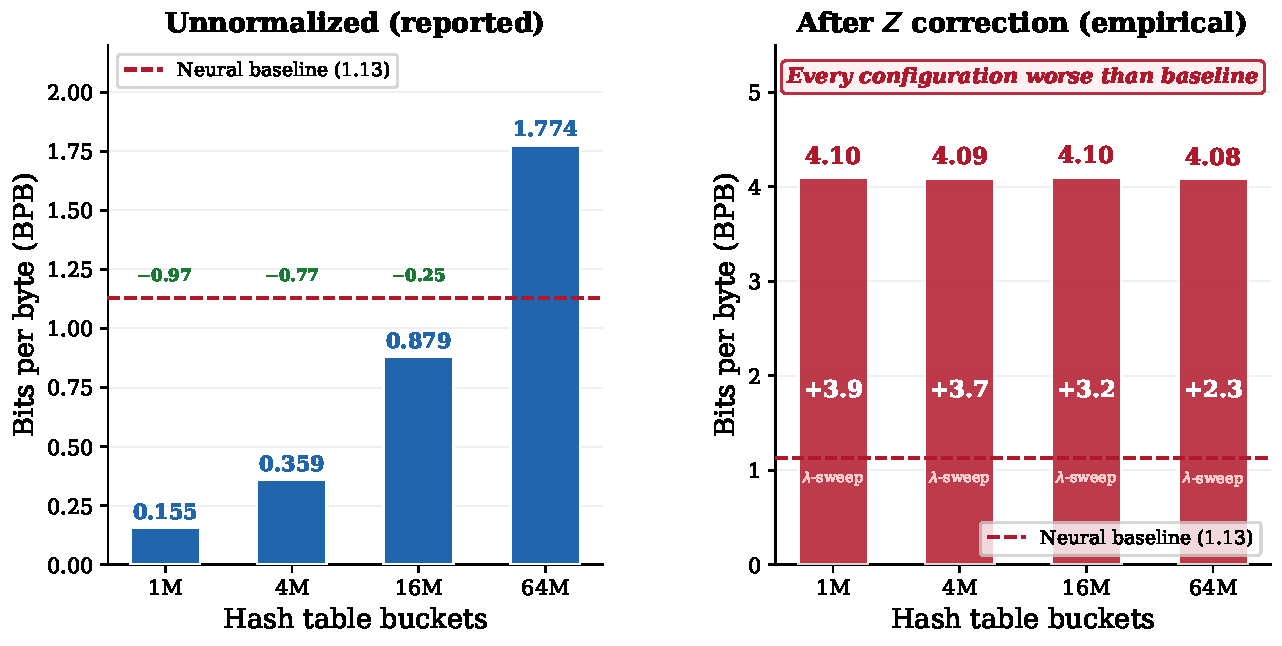
\includegraphics[width=\textwidth]{fig2_normalization.pdf}
\caption{The partition function correction eliminates the apparent improvement at all four bucket sizes ($\alpha = 2$). \emph{Left:} unnormalized BPB as reported in competition (smaller tables appear much better). \emph{Right:} after dividing by empirically measured $Z$, all four configurations produce BPB far above the 1.13 neural baseline. The $Z$ penalty (shown inside each bar) ranges from 2.3 to 3.9 bits per byte.}
\label{fig:normalization}
\end{figure}

\subsection{Recursive contractiveness}

Throughout Sections~\ref{sec:experiments}--\ref{sec:consequences}, we use a shared concentration $\alpha_n = \alpha$ for all orders (dropping the subscript) unless otherwise noted. The propagation weight $\gamma = \alpha/(c_{\text{obs}} + \alpha)$ determines how much lower-order $Z$ values influence higher orders. At 1M buckets with $\alpha = 2$: $\gamma \approx 0.032$. Each step attenuates the lower-order contribution by 97\%. After 2 steps, lower-order contributions are attenuated by $\gamma^2 \approx 0.001$. The final $Z$ is dominated by the highest order.

% ====================================================================
\section{Experimental Evidence}
\label{sec:experiments}

Unless otherwise noted, experiments use a 27M-parameter transformer trained with complementary n-gram loss (seed 1337)---a multitask objective that adds an auxiliary loss encouraging the model's hidden states to predict n-gram cache scores, so the neural model and cache work better together during training---evaluating on 62M tokens of FineWeb validation data with BPE-1024 ($V = 1024$). The neural-only baseline (cache disabled) achieves 1.130 BPB. Hash tables use 6 recursive n-gram orders (2--7). Selected key results are validated across two additional model seeds (2026, 415); see the multi-seed analysis in Section~\ref{sec:limitations}.

\subsection{Bucket-count sweep (36 configurations)}

We evaluate all combinations of 4 bucket counts $\times$ 9 concentration values:
\begin{itemize}
\item Buckets $B \in \{1\text{M}, 4\text{M}, 16\text{M}, 64\text{M}\}$, load factors $L \in \{59, 15, 4, 0.9\}$
\item Concentration $\alpha \in \{0.1, 0.5, 1.0, 2.0, 5.0, 10, 50, 100, 500\}$
\end{itemize}
Table~\ref{tab:exp1} additionally includes 131K buckets ($L \approx 500$) from a supplementary experiment at $\alpha = 2$ to show the trend at extreme load factors.

\begin{table}[h]
\centering
\caption{BPB at $\alpha = 2.0$ across 5 bucket sizes (see also Figure~\ref{fig:monotonic}).}
\label{tab:exp1}
\begin{tabular}{lccc}
\toprule
Buckets & Load Factor $L$ & BPB (unnorm.) & vs Neural (1.130) \\
\midrule
131K & $\sim$500 & 0.052 & $-$1.078 \\
1M & $\sim$59 & 0.155 & $-$0.975 \\
4M & $\sim$15 & 0.359 & $-$0.771 \\
16M & $\sim$4 & 0.879 & $-$0.251 \\
64M & $\sim$1 & 1.774 & $+$0.644 \\
\bottomrule
\end{tabular}
\end{table}

The ordering is monotonic across nearly 3 orders of magnitude in load factor (Figure~\ref{fig:monotonic}). At high load factors ($L \geq 4$), all bucket sizes share optimal $\alpha \approx 2.0$. At 64M buckets ($L \approx 1$), the optimum shifts to $\alpha \approx 10$. With low load factor the cache evidence is sparse and noisy ($c_{\text{obs}} \approx 2$ for singletons), so higher $\alpha$ improves performance by giving more weight to the (better-calibrated) neural prior. The full 36-configuration heatmap (Figure~\ref{fig:heatmap}) shows that $1\text{M} < 4\text{M} < 16\text{M} < 64\text{M}$ at every $\alpha$ tested---a sign test on the 3 adjacent pairs across 9 $\alpha$ values gives $p < (1/2)^9 < 0.002$ per pair, with all 27 comparisons in the predicted direction.

\begin{figure}[t]
\centering
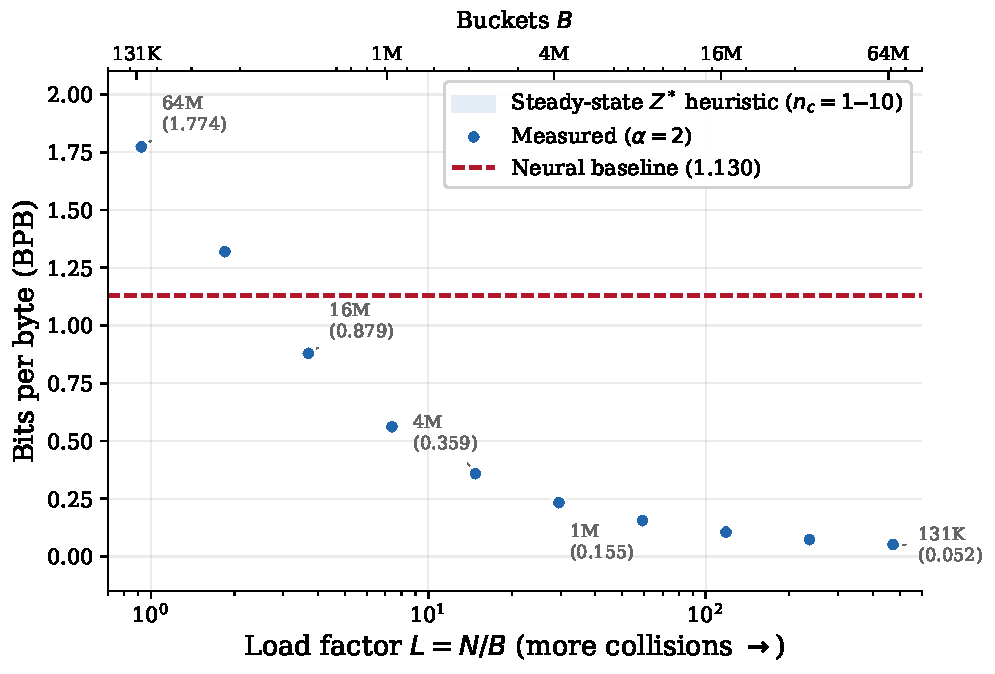
\includegraphics[width=0.7\textwidth]{fig1_bpb_vs_buckets.pdf}
\caption{BPB (unnormalized) vs.\ bucket count at $\alpha = 2$. The monotonic decrease with increasing load factor is consistent with the $Z^*$ scaling in~\eqref{eq:z_star}. Shaded band: steady-state $Z^*$ heuristic for $n_c \in [1, 10]$ (overestimates early-trajectory $Z$, so overestimates improvement). Dashed line: neural-only baseline (1.130 BPB).}
\label{fig:monotonic}
\end{figure}

\begin{figure}[t]
\centering
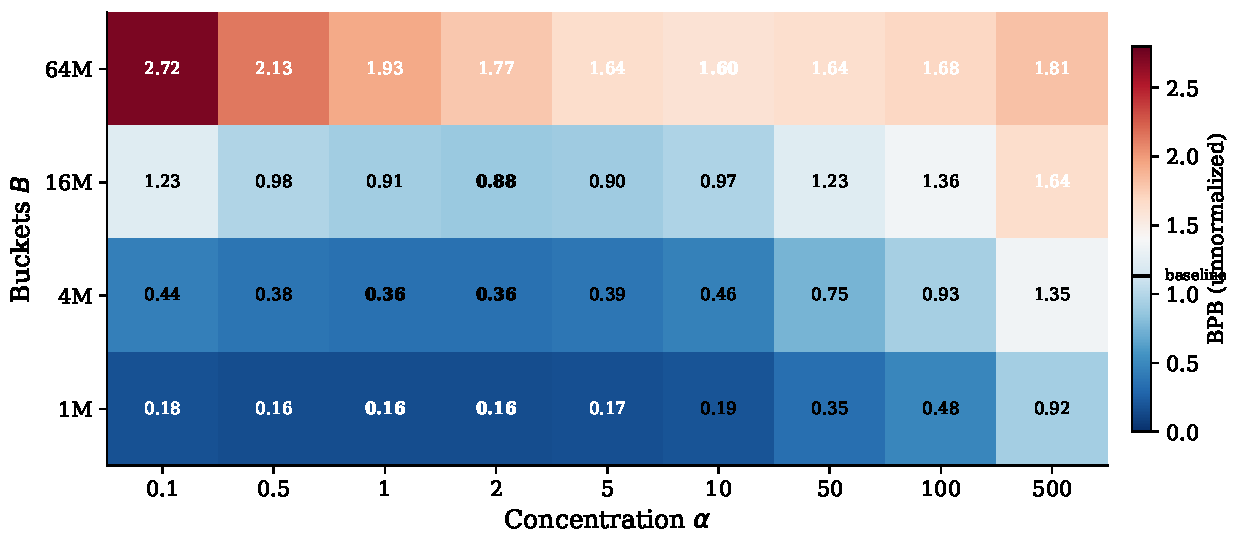
\includegraphics[width=0.8\textwidth]{fig3_alpha_heatmap.pdf}
\caption{BPB across 36 configurations (4 bucket sizes $\times$ 9 concentration values). The ordering $1\text{M} < 4\text{M} < 16\text{M} < 64\text{M}$ holds at every $\alpha$ tested.}
\label{fig:heatmap}
\end{figure}

\subsection{Per-order concentration profiles (27 configurations)}

A potential confound: the bucket-count effect might be an artifact of a single shared concentration parameter being suboptimal at different bucket sizes. If the optimal $\alpha$ differs across n-gram orders (plausible, since higher orders have sparser counts), a shared $\alpha$ could systematically disadvantage large tables.

To test this, we evaluate 6 per-order concentration profiles across 4 bucket sizes, plus 2 diagnostic profiles at selected bucket sizes (27 configurations total). Profiles range from uniform ($\alpha_k = 2$ for all $k$) to inverse-OBCL (low concentration at low orders, high at high orders) to extreme values ($\alpha = 10{,}000$).

The 1M-bucket configuration achieves the lowest BPB at every profile tested. The best profile (inverse-OBCL) achieves 0.153 at 1M, marginally better than uniform (0.155), while 64M with the same profile scores 1.589. Even at extreme concentration ($\alpha = 10{,}000$ at 1M, which should suppress most cache influence), the result is 1.493---still 0.36 points \emph{above} (worse than) the 1.130 neural baseline, consistent with $Z$ inflation persisting regardless of concentration tuning. This makes concentration mismatch an unlikely explanation for the bucket-count effect.

\subsection{Collision structure control}

Three conditions at matched $\alpha = 2$:
\begin{enumerate}
\item \textbf{Real 1M:} Standard XOR-prime hashing (natural collisions)
\item \textbf{Random-remap 1M:} Hash into 64M buckets, remap to 1M via random mapping (same collision \emph{rate}, random collision \emph{partners})
\item \textbf{Clean 64M:} Standard hashing with 64M buckets (minimal collisions)
\end{enumerate}

\begin{table}[h]
\centering
\caption{Collision structure experiment. Random collisions replicate 99.4\% of the observed BPB gap. The random-remap result is the mean $\pm$ std over 8 independent remap seeds (range: 0.16395--0.16406).}
\label{tab:exp3}
\begin{tabular}{lccc}
\toprule
Condition & BPB & Load Factor & Collision Structure \\
\midrule
Real 1M & 0.155 & $\sim$59 & Natural (linguistically correlated) \\
Random-remap 1M & $0.164 \pm 0.00004$ & $\sim$59 & Random (uncorrelated, 8 seeds) \\
Clean 64M & 1.774 & $\sim$1 & Minimal \\
\bottomrule
\end{tabular}
\end{table}

The gap between real and random collisions is just 0.009 BPB on a span of 1.619 BPB ($1 - 0.009/1.619 = 99.4\%$). Across 8 independent remap seeds, the random-remap BPB is $0.16401 \pm 0.00004$ (std), with a total range of 0.00012 BPB. This near-zero variance across remap seeds indicates that, in this configuration, the specific collision partners contribute negligibly: the collision \emph{rate} dominates. If collision-partner structure were the primary driver of the apparent improvement, we would expect random remapping---which preserves collision rate but destroys linguistic correlation between collision partners---to substantially degrade performance relative to real collisions. Instead, the gap is negligible and highly reproducible across remap instantiations.

\subsection{Synthetic floor control}

At 64M buckets (minimal real collisions), we add a fixed floor count $f_{\text{floor}}$ to every bucket in both context and full hash tables before evaluation. This drives $Z$ toward $V$ as the floor dominates real counts.

\begin{table}[h]
\centering
\caption{Synthetic floor at 64M buckets.}
\label{tab:synfloor}
\begin{tabular}{lcc}
\toprule
Floor & BPB & vs 64M Baseline (1.774) \\
\midrule
0 & 1.774 & --- \\
10 & 0.067 & $-$1.707 \\
30 & 0.032 & $-$1.742 \\
60 & 0.020 & $-$1.754 \\
\bottomrule
\end{tabular}
\end{table}

A floor of 60 at 64M achieves 0.020 BPB---lower than 131K real buckets (0.052)---even though the added floor counts carry zero linguistic information. The real 64M counts are still present but overwhelmed by the uniform floor. If the apparent BPB gains reflected predictive signal, adding uninformative counts would be expected to degrade performance; instead, it produces the lowest BPB in our entire study. This is consistent with the BPB improvement being driven by count-mass inflation of $Z$, not by the informational content of the cached counts.

\subsection{Sanity checks}

\begin{table}[h]
\centering
\caption{Validation controls.}
\label{tab:sanity}
\begin{tabular}{llcl}
\toprule
Check & Config & Result & Status \\
\midrule
Cache off & --- & 1.130 & Neural baseline \\
Order 3 only & 1M, $\alpha$=2 & 1.546 & Sparse n-grams hurt \\
Order 7 & 1M, $\alpha$=2 & 0.155 & Monotonic improvement \\
Dirichlet $\equiv$ interp. & 4M, $\alpha$=50 & 0.75420131 vs 0.75420131 & Identity to 8 d.p.\ (same run, two code paths) \\
Alt. hash primes & 4M, $\alpha$=50 & 0.747 vs 0.754 & Gap = 0.007 BPB \\
$\alpha = 1000$, 1M & 1M & 1.120 & Near-baseline \\
\bottomrule
\end{tabular}
\end{table}

% ====================================================================
\section{Consequences}
\label{sec:consequences}

\subsection{Normalization eliminates the apparent improvement in tested configurations}

Direct measurement of $Z_j = \sum_t p_K(t)$ at sampled positions shows that none of the four tested bucket-size configurations improves over the neural baseline under post-hoc normalization (Table~\ref{tab:normalized}). The normalization penalty, validated by the $\lambda$ sweep (Section~\ref{sec:lambda}), ranges from 2.31 (64M buckets) to 3.94 (1M buckets) BPB, yielding corrected BPB values of 4.08--4.10, all far above the 1.13 neural baseline. The measured $Z_{\max} = 1{,}024 \lesssim V$ at 1M buckets is consistent with the steady-state fixed point of the recurrence.

\paragraph{Two forms of normalization.} Our $Z$ correction divides the final output $p_K(t)$ by $Z_K = \sum_t p_K(t)$ after all recursive steps---\emph{post-hoc normalization}. An alternative is \emph{step-wise normalization}, which defines a separate recursion in which each intermediate is normalized before being passed as the prior to the next order. Setting $r_1(t) = \pi(t)$ and requiring $\sum_t r_n(t) = 1$ at every level gives:
\begin{equation}
r_n(t) = \frac{f_t^{(n)} + \alpha \cdot r_{n-1}(t)}{S^{(n)} + \alpha} = g_n(t) + \eta_n \, r_{n-1}(t)
\label{eq:stepwise}
\end{equation}
where $g_n(t) = f_t^{(n)}/(S^{(n)} + \alpha)$ is the normalized hashed-count contribution and $\eta_n = \alpha/(S^{(n)} + \alpha)$ is the prior-retention weight. Unrolling over $K - 1$ cache steps gives:
\[
r_K(t) = g_K(t) + \eta_K \, g_{K-1}(t) + \cdots + \Big(\prod_{m=2}^{K} \eta_m\Big) \pi(t).
\]
In the collision-heavy regime, $S^{(n)} \approx n_c + VL \gg \alpha$, so $\eta_n$ is tiny (e.g.\ $\eta \approx 2/60{,}400 \approx 3 \times 10^{-5}$ at 1M buckets with $\alpha = 2$). The neural prior's contribution is attenuated by $\prod_{m=2}^K \eta_m$, which effectively vanishes after one cache step. The final predictor can become dominated by $g_K(t)$---the normalized hashed-count distribution of the highest active order---which approaches uniformity when collision noise swamps the true count signal.

As a case study, we test step-wise normalization at 1M buckets ($\alpha = 2$, 6 orders), obtaining 4.15 BPB---far worse than the 1.13 neural baseline. PR~\#978 (AnirudhRahul) independently reported 1.51 BPB using a related approach: dividing by summed hashed-vocabulary mass at the final order. Both methods normalize by $S^{(n)} + \alpha$; the difference in outcomes (1.51 vs 4.15) arises from PR~\#978's different model architecture and single-order application rather than a different normalization principle. The three regimes are shown in Table~\ref{tab:three_regimes}.

\begin{table}[h]
\centering
\caption{Three normalization regimes at 1M buckets, $\alpha = 2$.}
\label{tab:three_regimes}
\begin{tabular}{lcc}
\toprule
Regime & BPB (1M) & vs Baseline \\
\midrule
Unnormalized (competition) & 0.155 & $-$0.975 \\
Step-wise normalized (ours, 6 orders) & 4.150 & $+$3.02 \\
Post-hoc $\div Z_K$ ($\lambda = 1$, Table~\ref{tab:lambda}) & 4.099 & $+$2.97 \\
Neural only & 1.130 & 0.00 \\
\bottomrule
\end{tabular}
\end{table}

Step-wise normalization (4.15) and post-hoc normalization (4.10) produce comparable BPB, both far worse than the neural baseline. Step-wise normalization introduces \emph{prior attenuation}: because $\eta_n \approx 3 \times 10^{-5}$, each recursive step nearly erases the information from all lower orders, leaving the predictor dominated by the noisy hashed-count distribution of the highest order. Under either normalization, the cache degrades performance relative to the neural baseline in our experiments: the apparent improvement exists only in the unnormalized scoring regime.

\subsection{Partial normalization interpolation}
\label{sec:lambda}

The jump from unnormalized (0.155 BPB) to post-hoc normalized (4.10 BPB) is large. To trace the transition smoothly, we interpolate between regimes using a partial normalization parameter $\lambda \in [0, 1]$. At each evaluation position $j$ where the cache has non-trivial counts (at least one n-gram order with context count $>0$), we divide the score by $Z_j^\lambda$:
\[
\text{score}_\lambda(t_j) = \begin{cases} p_K(t_j) / Z_j^\lambda & \text{if position } j \text{ has cache counts} \\ p_K(t_j) & \text{otherwise} \end{cases}
\]
where $\lambda = 0$ recovers the unnormalized competition score and $\lambda = 1$ gives the fully normalized probability at cache-active positions. The per-position $Z_j$ is computed by summing the Dirichlet-smoothed score over all $V = 1024$ vocabulary tokens (the same procedure as Section~\ref{sec:theory}, applied token-by-token). Since $Z_j$ is computed once from the unnormalized scores and does not depend on $\lambda$, the correction at cache-active positions decomposes exactly:
\begin{equation}
\text{BPB}_\lambda = \text{BPB}_0 + \frac{\lambda}{N_{\text{bytes}}} \sum_{j \in \mathcal{C}} \log_2 Z_j
\label{eq:lambda}
\end{equation}
where $\mathcal{C} = \{j : c^{(n)}_j > 0 \text{ for at least one order } n\}$ is the set of cache-active positions---those where at least one n-gram order has a nonzero context count, so the cache modifies the neural prediction. At 1M buckets, $|\mathcal{C}|/N_{\text{tok}} \approx 0.58$. Under fixed $Z_j$, linearity in $\lambda$ is an algebraic consequence of Eq.~\ref{eq:lambda}, not an empirical discovery. The 7-point measurement confirms this ($R^2 > 0.9999$); the useful output of the sweep is the slope (3.94) and the baseline crossover ($\lambda \approx 0.25$), not the linearity itself.

\begin{table}[h]
\centering
\caption{Partial normalization sweep at 1M buckets, $\alpha = 2$. BPB increases linearly with $\lambda$ (algebraically expected from Eq.~\ref{eq:lambda}). The apparent improvement over the 1.13 neural baseline vanishes by $\lambda \approx 0.25$. All values directly measured. Slope $\approx 3.94$ BPB per unit $\lambda$.}
\label{tab:lambda}
\begin{tabular}{ccc}
\toprule
$\lambda$ & BPB & vs Neural (1.13) \\
\midrule
0.0 & 0.155 & $-$0.975 \\
0.1 & 0.548 & $-$0.582 \\
0.2 & 0.941 & $-$0.189 \\
0.3 & 1.333 & $+$0.203 \\
0.5 & 2.119 & $+$0.989 \\
0.7 & 2.916 & $+$1.786 \\
1.0 & 4.099 & $+$2.969 \\
\bottomrule
\end{tabular}
\end{table}

The measurements (Table~\ref{tab:lambda}, Figure~\ref{fig:lambda}) confirm the expected linearity, with measured slope $\approx 3.94$ BPB per unit $\lambda$. From Equation~\ref{eq:lambda}, this slope equals $(1/N_{\text{bytes}}) \sum_{j \in \mathcal{C}} \log_2 Z_j$: the byte-weighted sum of $\log_2 Z$ over cache-active positions. The crossover point---where cache BPB exceeds the 1.13 neural baseline---occurs near $\lambda \approx 0.25$: even 25\% normalization erases the apparent gain.

\paragraph{$\lambda$-sweep as ground truth for the normalization penalty.} The $\lambda = 1.0$ result (4.10 BPB) directly measures the post-hoc normalized BPB, because dividing by $Z_j^1 = Z_j$ at each cache-active position is exactly post-hoc normalization. This value is lower than one might compute from the naive formula $\bpb_{\text{unnorm}} + \rho \cdot \E[\log_2 Z] = 0.155 + 0.71 \times 9.61 = 6.98$, where $\E[\log_2 Z] = 9.61$ is the sampled conditional average over cache-active positions from Table~\ref{tab:normalized}. The discrepancy (factor $\approx 0.58$) arises primarily because only $|\mathcal{C}|/N_{\text{tok}} \approx 0.58$ of token positions are cache-active; the naive formula applies the conditional average $\E[\log_2 Z \mid j \in \mathcal{C}]$ to \emph{all} positions, overstating the penalty by a factor of $1/0.58 \approx 1.72$. Correcting for this: $0.58 \times 0.71 \times 9.61 = 3.96 \approx 3.94$, matching the $\lambda$-sweep slope. The $\lambda$-sweep slope provides the correct per-byte penalty directly, without requiring knowledge of the cache-active fraction. We validated the $\lambda$ sweep at a second bucket size: at 64M buckets, $\lambda = 0.5$ yields BPB $= 2.929$, giving slope $= 2 \times (2.929 - 1.774) = 2.31$, consistent with Table~\ref{tab:normalized}'s 64M penalty.

\begin{figure}[h]
\centering
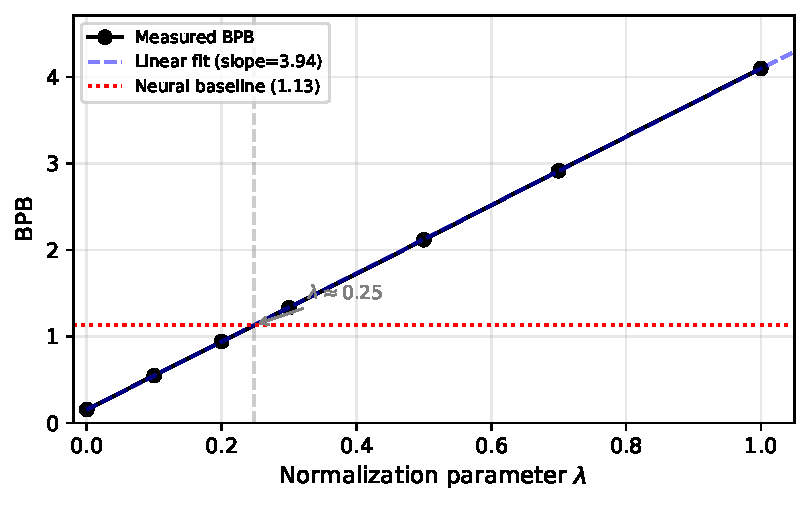
\includegraphics[width=0.75\textwidth]{fig_lambda_sweep.pdf}
\caption{BPB vs.\ partial normalization $\lambda$ (1M buckets, $\alpha = 2$, seed 1337). Linearity follows from Eq.~\ref{eq:lambda}; the dashed red line marks the 1.13 neural baseline. The crossover at $\lambda \approx 0.25$ means that 25\% normalization eliminates the apparent improvement. Slope $\approx$ 3.94 BPB per unit $\lambda$.}
\label{fig:lambda}
\end{figure}

\subsection{Cross-submission normalization evidence}

Our normalization diagnosis is corroborated by two independent submissions. PR~\#978 (AnirudhRahul) identified the same denominator bug in a hashed n-gram cache: replacing the context count with the summed hashed-vocabulary mass degraded performance from 0.39 to 1.51 BPB. The author confirmed: ``the entire n-gram gain is collision artifact.'' Our order-3-only result at 1M buckets (1.546 BPB) closely matches this 1.51, consistent with single-order normalization producing similar outcomes across implementations.

Separately, PR~\#511 (AnirudhRahul) implemented a collision-free delayed PPM model using exact trie counts with a 2048-token delay (ensuring no overlap with the transformer's sliding window). With proper normalization and exact counts, the n-gram cache improved by $-0.00126$ BPB (from 1.143 to 1.142, std $= 0.00002$ across 3 seeds). This demonstrates that exact n-gram statistics can provide a genuine, reproducible improvement---but the magnitude is $0.0013$ BPB, roughly ${\sim}775\times$ smaller than the 0.975-point apparent gain from unnormalized hashed caches. These external results are not controlled comparisons, but provide independent qualitative agreement with the normalization-based explanation. (PR~\#511 uses a different model architecture and a 2048-token delay, so the baselines differ slightly.)

\subsection{Pitman-Yor discount degrades performance}

With PY discount $d$, the effective count becomes $\max(f - d, 0)$, reducing $S$. Since $Z^* = S/c$, the discount shrinks $Z$, reducing score inflation. Under the unnormalized metric, anything that reduces $Z$ hurts. Degradation is monotonic: $d = 0$ (pure Dirichlet) is optimal. (We fit a Zipf-Mandelbrot distribution $p(r) \propto (r + q)^{-s}$ to the BPE-1024 unigram frequencies on FineWeb and obtain $s = 0.86 < 1$, consistent with a flatter unigram distribution than standard Zipf. This provides supportive intuition but not a standalone proof.)

\subsection{Why unnormalized scoring was standard}

Among the cache-augmented submissions we reviewed (PRs \#777, \#796, \#834, \#900, \#913, \#986, \#1114), none computes the full normalized distribution. The competition metric evaluates only the true token's score, so there is no incentive to compute $Z$.

\subsection{Practical implications}

For practitioners implementing hashed n-gram caches:
\begin{enumerate}
\item \textbf{Always normalize.} If your system uses cached count scores, divide by $Z$ or track $\log Z$ alongside $\log p(t)$.
\item \textbf{$Z$ as a diagnostic.} The fixed-point formula provides a quick check: if $(n_c + VL)/(n_c + L) \gg 1$, unnormalized scores are unreliable.
\item \textbf{After normalization, fewer collisions are better (in our tests).} Once $Z$ is corrected, larger hash tables gave better estimates in all four tested configurations.
\end{enumerate}

% ====================================================================
\section{Negative Results}

\begin{table}[h]
\centering
\caption{Negative results, with $Z$-based explanations where applicable.}
\label{tab:negative}
\begin{tabular}{lll}
\toprule
Approach & Result & Explanation via $Z$ \\
\midrule
PY discount $d > 0$ & Monotonic degradation & Reduces $S \to$ reduces $Z$ \\
Modified Kneser-Ney & Large degradation & Assumes reliable counts; collisions violate this \\
Context Tree Weighting & Large degradation & Requires proper normalization internally \\
Test-time training & No improvement on our stack & Adapts neural model; does not affect cache $Z$ \\
Higher orders ($>$7) & Diminishing returns & $Z$ already near $Z^*$ after 2--3 steps \\
\bottomrule
\end{tabular}
\end{table}

The $Z$ mechanism explains why approaches that reduce count mass $S$ (PY discount) or require properly normalized inputs (MKN, CTW) fail in this setting. For the remaining approaches, $Z$ is consistent with the observed outcomes but we do not claim it is the sole explanatory factor.

% ====================================================================
\section{Related Work}

\paragraph{Interpolated smoothing.} \citet{chen1999empirical} provided the foundational empirical study of smoothing techniques for n-gram language models, including modified Kneser-Ney and interpolated backoff. Our recursive Dirichlet-multinomial mixing (Eq.~\ref{eq:recursion}) is algebraically equivalent to interpolated backoff with weight $\lambda_n = c^{(n)}/(c^{(n)} + \alpha_n)$. The key difference is that our counts are corrupted by hash collisions, which inflates $S$ and therefore $Z$.

\paragraph{Neural and retrieval-augmented caches.} \citet{grave2017improving} introduced the continuous neural cache, which interpolates a neural LM with a non-parametric cache over recent hidden states. \citet{khandelwal2020generalization} extended this idea with $k$-nearest-neighbor language models (kNN-LM), retrieving from a datastore of cached hidden states at inference time. Both approaches store exact representations and avoid hash collisions entirely; our analysis is specific to the hashed count-based variant where collisions inflate the partition function. \citet{grave2017improving} also found that global normalization of the cache mixture slightly hurt perplexity (74.9 vs.\ 74.6), an early hint that unnormalized cache scoring can inflate apparent gains.

\paragraph{Self-normalization and partition functions.} \citet{devlin2014fast} showed that neural LMs can be trained to be approximately \emph{self-normalizing} ($\log Z \approx 0$), avoiding the cost of computing the full softmax. \citet{andreas2015when} proved conditions under which log-linear models achieve self-normalization and showed that deviations from $Z = 1$ correlate with model error. In noise-contrastive estimation \citep{mnih2012fast}, the partition function is explicitly modeled as a learnable parameter rather than ignored. The $Z$ inflation we observe is an extreme case of non-self-normalization: the hashed count recursion drives $Z$ above 1,000, three orders of magnitude beyond the deviations studied in the self-normalization literature. Our practical recommendation---always compute $Z$---parallels the NCE insight that the partition function cannot be neglected.

\paragraph{Hierarchical Bayesian LMs.} \citet{teh2006hierarchical} developed hierarchical Pitman-Yor language models (HPYLM), which provide the Bayesian foundation for interpolated n-gram smoothing. Our Dirichlet-multinomial recursion (Eq.~\ref{eq:recursion}) is a special case of this framework with $d = 0$. HPYLM assumes exact counts; our counts are corrupted by hash collisions, creating the $Z$ inflation we analyze.

\paragraph{Randomized language models.} \citet{talbot2007smoothed} studied Bloom filter-based language models for space-efficient storage. Their work focuses on trained model compression, not emergent properties of hash collisions in transductive caching.

\paragraph{Hash kernels.} \citet{weinberger2009feature} proved that signed random hash projections preserve inner products in expectation. Their analysis requires sign bits $\xi(j) \in \{\pm 1\}$ for unbiasedness. Our hash tables are unsigned positive accumulators where collisions create one-sided positive bias, so the Weinberger bounds do not transfer.

\paragraph{Approximate counting and Bayesian nonparametric sketching.} The count-min sketch (CMS) \citep{cormode2005improved} is the standard data structure for approximate frequency estimation in streams. \citet{cai2018bayesian} gave a Bayesian nonparametric interpretation of CMS queries using a Dirichlet process prior. Our recursion (Eq.~\ref{eq:recursion}) can be viewed as a hierarchical version of this framework applied across n-gram orders, where each level compounds the one-sided collision bias that \citet{cai2018bayesian} characterized for a single sketch.

\paragraph{Collision-free hashing.} \citet{lin2026engram}, in a controlled study of Engram-style conditional memory \citep{cheng2026engram}, found that replacing collision-prone hashing with a collision-free hot tier does not improve validation loss, consistent with our finding that in our tested setting, collision structure plays a smaller role than count-inflation magnitude.

\paragraph{Dirichlet-multinomial smoothing in compression benchmarks.} The application of Dirichlet-multinomial smoothing to hashed n-gram caches in the Parameter Golf setting was introduced in PR~\#796 (March~26, 2026), replacing ad-hoc per-order multipliers with a single concentration parameter. Subsequent work (PR~\#986) built on this framework. The present paper identifies the partition function inflation mechanism in this class of systems.

% ====================================================================
\section{Limitations and Future Work}
\label{sec:limitations}

\paragraph{Reproducibility.} All experiments use \texttt{train\_gpt\_ngram\_v4\_5\_phrase\_perorder.py} in eval-only mode with the following environment variables: \texttt{EVAL\_ONLY=1}, \texttt{NGRAM\_CACHE=1}, \texttt{NGRAM\_DIRICHLET=1}, \texttt{NGRAM\_MIN\_ORDER=2}, \texttt{NGRAM\_ORDER=7}, \texttt{EVAL\_STRIDE=64}, \texttt{MEASURE\_Z\_EVERY=10}. Per-experiment settings: bucket count via \texttt{NGRAM\_BUCKETS}, concentration via \texttt{NGRAM\_CONCENTRATION} or \texttt{NGRAM\_PER\_ORDER\_CONC}, normalization via \texttt{NORM\_LAMBDA} or \texttt{NORMALIZE\_STEPWISE=1}, random remap via \texttt{NOISE\_CONTROL\_BUCKETS} and \texttt{NOISE\_CONTROL\_SEED}, synthetic floor via \texttt{SYNTHETIC\_FLOOR}. The Dirichlet recursion path is not the script's default; it requires \texttt{NGRAM\_DIRICHLET=1}. All reported numbers use these explicit overrides.

\paragraph{Scope and non-claims.} This paper analyzes one specific mechanism---partition function inflation under unnormalized scoring---in one specific system class: hashed count-based n-gram caches with Dirichlet-multinomial smoothing, evaluated on BPE-1024 FineWeb data. We do not claim that all cache-augmented language models fail under normalization, that collision structure never carries useful information, or that hashed n-gram statistics are inherently useless for language modeling. Our results are specific to the unnormalized transductive evaluation setting studied here. Whether properly normalized cache systems could improve over neural baselines under different architectures, hash schemes, or vocabulary sizes remains an open question.

\paragraph{Three model seeds.} We have validated the main results across three independently trained neural models (seeds 1337, 2026, and 415). All hit the 10-minute wallclock cap at different step counts (1793, 5440, and 1794 respectively, due to different hardware configurations), yielding different neural baselines (1.130, 1.152, and 1.272 BPB). Despite this spread in neural quality, the cache produces near-identical behavior:

\begin{center}
\small
\begin{tabular}{lccc}
\toprule
Seed & Buckets & BPB & $\Delta$ from 1337 \\
\midrule
1337 & 1M & 0.15536 & --- \\
2026 & 1M & 0.15538 & +0.00002 \\
415 & 1M & 0.15563 & +0.00027 \\
\midrule
1337 & 64M & 1.77346 & --- \\
2026 & 64M & 1.77355 & +0.00009 \\
415 & 64M & 1.77480 & +0.00134 \\
\bottomrule
\end{tabular}
\end{center}

\noindent At 1M buckets, cross-seed deltas are $<$0.0003 BPB despite a 142 mBPB spread in neural baselines---comparable to the 8-seed remap variance ($\text{std} = 0.00004$). At 64M buckets the delta is slightly larger (0.0013 BPB), consistent with the neural prior having more influence at low load factor ($L \approx 1$). Both are negligible relative to the effect sizes in Table~\ref{tab:exp1}, supporting the conclusion that, in our three-seed test, the cache score is nearly insensitive to neural model seed and far more sensitive to hash-table configuration.

\subsection{Scaling to production vocabulary sizes}
\label{sec:scaling}

Our experiments use BPE-1024 ($V = 1024$), an unusually small vocabulary dictated by the competition constraints. Modern language models use $V = 32{,}000$ (LLaMA, Mistral), $V = 50{,}257$ (GPT-2), or $V = 128{,}000$ (GPT-4). Since the fixed point $Z^* = (n_c + VL)/(n_c + L)$ scales linearly with $V$ in the high-load regime ($VL \gg n_c$), the partition function inflation diagnosed here becomes \emph{more severe}, not less, at production vocabulary sizes.

\paragraph{Projected $Z^*$ at standard vocabularies.} For singleton contexts ($n_c = 1$) at a representative load factor $L = 59$ (corresponding to 1M buckets with 62M tokens, our primary experimental setting):

\begin{table}[h]
\centering
\caption{Projected partition function inflation at production vocabulary sizes ($n_c = 1$, $L = 59$). The BPB penalty is $\rho \cdot \log_2 Z^*$, with $\rho = 0.71$ (our measured tokens-per-byte ratio; production tokenizers with larger $V$ will have different $\rho$, typically lower, partially offsetting the larger $Z^*$). These projections use only the fixed-point formula~\eqref{eq:z_star} with no additional approximations.}
\label{tab:scaling}
\begin{tabular}{lrrrl}
\toprule
Vocabulary & $V$ & $Z^*$ & $\log_2 Z^*$ & Context \\
\midrule
BPE-1024 (this paper) & 1,024 & 1,007 & 10.0 & Parameter Golf \\
BPE-4K & 4,096 & 4,028 & 12.0 & Small LMs \\
BPE-32K & 32,000 & 31,467 & 14.9 & LLaMA, Mistral \\
BPE-50K & 50,257 & 49,419 & 15.6 & GPT-2 \\
BPE-128K & 128,000 & 125,867 & 17.0 & GPT-4 \\
\bottomrule
\end{tabular}
\end{table}

\noindent At $V = 32{,}000$, the partition function exceeds 31,000---meaning the scoring function's outputs would sum to ${\sim}31{,}000$ instead of 1. The $\log_2 Z^*$ penalty grows from 10.0 bits per token (our setting) to 14.9 bits per token. Any system that (i)~uses hashed count tables, (ii)~applies a Dirichlet-style recursive update, and (iii)~evaluates only the true token's unnormalized score will face this inflation, with severity proportional to $V$.

\paragraph{Why $V$ matters mechanically.} The inflation arises because each of $V$ tokens is looked up in an independent full-table bucket, and the collision noise in each bucket contributes additively to $S = \sum_t f_t^{(n)}$. With $V$ independent lookups each contributing ${\sim}L$ collision counts, $S \approx n_c + VL$ while the context count remains $c_{\text{obs}} = n_c + L$. The ratio $S/c_{\text{obs}}$ therefore scales as ${\sim}V$ when $VL \gg n_c$. Larger vocabularies do not reduce the collision noise---they \emph{amplify} it, because there are more buckets contributing spurious counts to the sum.

\paragraph{Partial offsetting factors.} Two factors partially offset the larger $Z^*$ at production scale. First, production tokenizers with larger $V$ typically achieve lower tokens-per-byte ratios ($\rho \approx 0.25$--$0.35$ for BPE-32K vs.\ $\rho = 0.71$ for BPE-1024), reducing the BPB penalty per unit $\log_2 Z$. Second, production systems typically use larger hash tables (more memory budget), reducing $L$ and therefore $Z^*$. However, even at $L = 1$ (nearly collision-free) with $V = 32{,}000$: $Z^* = (1 + 32{,}000)/2 = 16{,}001$, still four orders of magnitude above 1. The load factor would need to drop below $L = 1/V \approx 3 \times 10^{-5}$ for $Z^*$ to approach 1---requiring hash tables with ${\sim}V \times N$ buckets, which defeats the purpose of hashing.

\paragraph{Diagnostic rule of thumb.} For any hashed count-based system with vocabulary $V$, bucket count $B$, $N$ evaluation tokens, and representative context count $n_c$: compute the steady-state fixed point $Z^* = (n_c + VL)/(n_c + L)$ where $L = N/B$. In the high-load regime ($L \gg 1$), $Z^*$ saturates at ${\approx}V$, giving $\log_2 V$ bits per token of inflation (10 bits at $V = 1{,}024$; 15 bits at $V = 32\text{K}$). In the low-load regime ($L \ll 1$), $Z^* \approx 1 + (V-1)L/(n_c + L)$, growing linearly in $L$. If $Z^* \gg 1$, unnormalized scores are unreliable regardless of the apparent BPB. Computing $Z$ exactly requires evaluating $p_K(t)$ for all $V$ tokens at each position---cheap at $V = 1{,}024$ but $32\times$ more expensive at $V = 32$K. A Monte Carlo estimate using a random subset of $V' \ll V$ tokens, scaled by $V/V'$, provides an approximation; we have not tested this but note that the smooth dependence of $Z$ on position (driven by load factor) suggests low variance.

\paragraph{Singleton upper bound.} The closed-form $Z^*$ with $n_c = 1$ overestimates the trajectory-averaged $\E[\log_2 Z]$ by roughly 4\% at 1M buckets ($L \approx 59$) but by roughly 40\% at 64M buckets ($L \approx 1$), because at low load factors, fewer contexts accumulate the large collision counts that drive $Z$ toward its fixed point. Using $n_c = 5$ matches the 1M measurement to within 0.3\%. A tighter bound could be derived from the empirical context-count distribution.

\paragraph{Lambda sweep at two bucket sizes.} The full 7-point partial normalization sweep (Section~\ref{sec:lambda}) is conducted only at 1M buckets, with a single bonus measurement at 64M buckets ($\lambda = 0.5$) confirming the slope prediction. Equation~\ref{eq:lambda} predicts that the same linear relationship should hold at any bucket size, with a different slope determined by that configuration's normalization penalty. A full per-position $\lambda$ sweep at each of the four bucket sizes remains future work.

\paragraph{No exact collision-free baseline.} Our cleanest low-collision condition is 64M buckets ($L \approx 1$). A minimal perfect hash function baseline would be cleaner; \citet{lin2026engram} found that collision-free hashing does not improve neural cache performance, consistent with our finding that in our tested setting, collision structure plays a smaller role than count-inflation magnitude (Section~\ref{sec:experiments}). The monotonic trend across nearly three orders of magnitude in $L$ (from $\sim$1 to $\sim$500) is consistent with continuous scaling of the effect.

\paragraph{Toward working cache systems.} Our analysis diagnoses why hashed caches fail under normalization but does not provide a constructive fix. Three directions merit investigation. First, \emph{debiased count estimators}: subtracting the expected collision contribution $L$ from each bucket count before computing the recursive score, analogous to bias correction in count-min sketches. Second, \emph{signed hashing}: using $\xi(j) \in \{+1, -1\}$ sign bits as in \citet{weinberger2009feature}, which produces $\E[S] = n_c$ (no positive bias) and should maintain $Z \approx 1$, though at the cost of allowing negative intermediate counts. Third, \emph{exact retrieval}: collision-free data structures such as the delayed PPM trie in PR~\#511, which achieves $Z = 1$ by construction but provides only 0.001 BPB genuine improvement in this setting. Whether any of these approaches can extract meaningful signal from n-gram statistics beyond what the neural model already captures remains an open question.

% ====================================================================
\section{Conclusion}

The apparent success of hashed n-gram caches in transductive compression benchmarks is largely attributable to partition function inflation under unnormalized scoring. The $Z$ recurrence $Z_n = (S^{(n)} + \alpha \cdot Z_{n-1})/(c^{(n)} + \alpha)$ provides an explanation of the main mechanism: smaller hash tables produce more collisions, inflating count totals $S$ and therefore $Z$, which lowers unnormalized log-probability scores without improving the underlying probability estimates.

Five lines of evidence support this diagnosis. First, the bucket-count ranking holds across all 36 configurations and 6 per-order profiles. Second, across 8 independent remap seeds, rate-matched random collisions replicate 99.4\% of the observed BPB gap with near-zero variance ($\text{std} = 0.00004$ BPB). Third, direct empirical measurement of $Z$ at four bucket sizes yields $\E[\log_2 Z]$ ranging from 5.6 (64M buckets) to 9.6 (1M buckets), with $Z_{\max} \lesssim V$ consistent with the steady-state fixed point. Fourth, a partial normalization sweep (Section~\ref{sec:lambda}) crosses the neural baseline at $\lambda \approx 0.25$, with the measured slope (3.94 BPB/$\lambda$) matching the prediction from Eq.~\ref{eq:lambda} after accounting for the cache-active fraction. Fifth, an independent collision-free trie (PR~\#511) achieves only $-0.0013$ BPB improvement---${\sim}775\times$ smaller than the 0.975-point unnormalized hash-based apparent gain---consistent with genuine collision-free gains being much smaller than the unnormalized hashed-cache artifact in at least one independent implementation.

The organizers' late March 2026 decision to close dozens of cache-augmented submissions aligns with this diagnosis. The $Z$ recurrence and empirical measurements provide a quantitative diagnostic for partition function inflation in hashed count-based systems.

% ====================================================================
\section*{Acknowledgements}

The author thanks the OpenAI Parameter Golf community for creating the empirical conditions that made this analysis possible. In particular: GitHub users Eppie and mhuen for identifying, in discussion on PR~\#900, that hash collisions break the normalization identity $\sum_t p(t) = 1$ even when the Dirichlet-multinomial formula is algebraically correct; sofiabod (PR~\#986) for extending the Dirichlet smoothing framework; AnirudhRahul (PR~\#978) for independently confirming the normalization gap; the competition organizers, especially valerio-oai, for the late March analysis and ruling that prompted this investigation; and the many participants whose cache submissions motivated this analysis. The author thanks OpenAI for organizing the Parameter Golf challenge and RunPod for providing GPU compute credits. Claude (Anthropic) was used for computational assistance and experiment automation.

\bibliographystyle{plainnat}
\bibliography{references}

% ====================================================================
\appendix

\section{Full Experimental Data}
\label{app:full_data}

\paragraph{Full $\alpha$ sweep (36 configurations).}

\begin{table}[h]
\centering
\small
\caption{Complete exp1 results. Bold = best per bucket size.}
\label{tab:full_sweep}
\begin{tabular}{l|ccccccccc}
\toprule
Buckets & $\alpha$=0.1 & 0.5 & 1.0 & 2.0 & 5.0 & 10 & 50 & 100 & 500 \\
\midrule
1M & 0.176 & 0.159 & 0.1555 & \textbf{0.1554} & 0.166 & 0.189 & 0.348 & 0.483 & 0.922 \\
4M & 0.441 & 0.376 & 0.360 & \textbf{0.359} & 0.392 & 0.456 & 0.754 & 0.930 & 1.346 \\
16M & 1.232 & 0.984 & 0.913 & \textbf{0.879} & 0.901 & 0.967 & 1.230 & 1.364 & 1.644 \\
64M & 2.717 & 2.134 & 1.930 & 1.774 & 1.645 & \textbf{1.603} & 1.637 & 1.685 & 1.807 \\
\bottomrule
\end{tabular}
\end{table}

\paragraph{Order ablation at 1M buckets, $\alpha = 2$.}

\begin{table}[h]
\centering
\caption{BPB saturates by order 7--9, consistent with $\gamma \approx 0.03$.}
\begin{tabular}{lcc}
\toprule
Max Order & BPB & Orders Used \\
\midrule
3 & 1.546 & 2--3 \\
5 & 0.369 & 2--5 \\
7 & 0.155 & 2--7 \\
9 & 0.117 & 2--9 \\
11 & 0.108 & 2--11 \\
15 & 0.103 & 2--15 \\
\bottomrule
\end{tabular}
\end{table}

\paragraph{Step-wise normalization vs.\ max order (1M buckets, $\alpha = 2$).}

Under step-wise normalization, adding more recursive orders worsens BPB because each additional step attenuates the neural prior by $\eta_n \approx 3 \times 10^{-5}$ (Section~\ref{sec:consequences}). Table~\ref{tab:stepwise_sweep} shows this degradation.

\begin{table}[h]
\centering
\caption{Step-wise normalized BPB increases with more recursive orders. Each additional order further attenuates the neural prior, replacing it with noisy hashed-count distributions.}
\label{tab:stepwise_sweep}
\begin{tabular}{lccc}
\toprule
Orders & Steps & BPB (step-wise) & vs Neural (1.130) \\
\midrule
2--3 & 2 & 3.417 & $+$2.287 \\
2--4 & 3 & 3.859 & $+$2.729 \\
2--5 & 4 & 4.047 & $+$2.917 \\
2--7 & 6 & 4.150 & $+$3.020 \\
\bottomrule
\end{tabular}
\end{table}

\paragraph{Reproducibility.} Quantitative results reported in the main tables and figures are derived from CSV files shipped with the source: \texttt{paper\_results\_local/exp1\_captured.csv} (36-configuration sweep), \texttt{z\_measurements.csv} (partition function measurements at 4 bucket sizes), \texttt{stepwise\_results.csv} (step-wise normalization), \texttt{exp3\_captured.csv} (collision control), \texttt{remap\_multiseed.csv} (8-seed remap results), and \texttt{bonus\_captured.csv} (supplementary experiments). The negative results in Table~\ref{tab:negative} are qualitative summaries from development experiments not included in these CSVs. The figure generation script reads the quantitative CSVs directly.

\section{Derivation Details}
\label{app:derivations}

\paragraph{Collision bias expectations.} Under uniform hashing with load factor $L$, each token $t$ is looked up in an independent full-table bucket:
\begin{align}
\E[f_t \mid \text{true count } k_t] &= k_t + L \\
\E[S] = \E\bigg[\sum_t f_t\bigg] &= n_c + V \cdot L \\
c_{\text{obs}} &= n_c + L
\end{align}

The expected bias for token $t$ is:
\[
\E[B_n(t)] = \frac{\E[f_t] - c_{\text{obs}} \cdot p_{\text{true}}(t)}{c_{\text{obs}} + \alpha} = \frac{k_t + L - (n_c + L) \cdot p_{\text{true}}(t)}{c_{\text{obs}} + \alpha}
\]

For the partition function, summing over all $V$ tokens: $\E[Z - 1] \approx L(V-1)/(c_{\text{obs}} + \alpha)$.

\paragraph{Fixed-point derivation.} Substituting the collision model into the $Z$ recurrence~\eqref{eq:z_recurrence}:
\[
Z_n = \frac{n_c + V \cdot L + \alpha \cdot Z_{n-1}}{n_c + L + \alpha}
\]
Setting $Z_n = Z_{n-1} = Z^*$ and solving:
\[
Z^*(c_{\text{obs}} + \alpha) = S + \alpha \cdot Z^* \implies Z^* \cdot c_{\text{obs}} = S \implies Z^* = \frac{S}{c_{\text{obs}}} = \frac{n_c + V \cdot L}{n_c + L}
\]
This is independent of $\alpha$: the concentration affects convergence rate but not the fixed point.

\paragraph{Contraction proof.} The recurrence $Z_n = \frac{S + \alpha \cdot Z_{n-1}}{c + \alpha}$ is an affine map with slope $\gamma = \alpha/(c + \alpha) < 1$. By the contraction mapping theorem, the sequence converges geometrically:
\[
|Z_n - Z^*| = \gamma \cdot |Z_{n-1} - Z^*| = \gamma^{n-1} \cdot |Z_1 - Z^*|
\]
At 1M buckets with $\alpha = 2$ and $c_{\text{obs}} \approx 60$: $\gamma = 2/62 \approx 0.032$. After two cache steps: $\gamma^2 \approx 0.001$, so $Z$ is within 0.1\% of $Z^*$.

\paragraph{Jensen's inequality note.} The normalization identity (Eq.~\ref{eq:bpb_norm}) is exact when the sum runs over all scored positions. Jensen's inequality becomes relevant only when approximating $\E[\log_2 Z]$ from the theoretical $\log_2 \E[Z]$: since $\log_2$ is concave, $\E[\log_2 Z] \leq \log_2 \E[Z]$, and the gap is bounded by the variance of $Z$. Over the evaluation trajectory, $Z$ varies smoothly (driven by load factor), giving a Jensen gap of at most 0.31 $\log_2$ units---small relative to $\E[\log_2 Z] \approx 10$.

\paragraph{Tokens-per-byte ratio.} BPB measures bits per byte, while the partition function inflates bits per token. With BPE-1024, our tokenizer produces $N_{\text{tok}} = 62{,}021{,}632$ tokens from $N_{\text{bytes}} = 87{,}386{,}893$ bytes of raw text. The ratio $\rho = N_{\text{tok}} / N_{\text{bytes}} \approx 0.71$ appears in the conversion from the per-token $Z$ penalty to the per-byte BPB penalty (Eq.~\ref{eq:bpb_norm}).

\section{Additional Theoretical Results}
\label{app:theorems}

\paragraph{Step-wise normalization recurrence.}
Under step-wise normalization (normalizing intermediates at each order so that $\sum_t r_n(t) = 1$), the recurrence is:
\[
r_n(t) = g_n(t) + \eta_n \, r_{n-1}(t), \qquad g_n(t) = \frac{f_t^{(n)}}{S^{(n)} + \alpha_n}, \quad \eta_n = \frac{\alpha_n}{S^{(n)} + \alpha_n},
\]
with $r_1(t) = \pi(t)$. Unrolling over $K - 1$ cache steps:
\[
r_K(t) = g_K(t) + \eta_K \, g_{K-1}(t) + \eta_K \eta_{K-1} \, g_{K-2}(t) + \cdots + \Big(\prod_{m=2}^{K} \eta_m\Big) \pi(t).
\]
The neural prior's weight is $\prod_{m=2}^K \eta_m$. At 1M buckets with $S^{(n)} \approx 60{,}400$ and $\alpha = 2$: $\eta \approx 3.3 \times 10^{-5}$. With $K = 7$ (six cache steps), the prior weight is $\eta^6 \approx 10^{-27}$, effectively zero. The final predictor can become dominated by $g_K(t)$, which distributes probability approximately as $f_t^{(K)} / S^{(K)}$---approaching uniformity when collision noise dominates.

\paragraph{Exact variable-coefficient recurrence.}
The closed-form~\eqref{eq:closed_form} assumes constant $\gamma_n \approx \gamma$. When per-order parameters differ, the exact solution is available. Writing the recurrence as
\[
Z_n = A_n + \gamma_n \, Z_{n-1}, \qquad A_n = \frac{S^{(n)}}{c^{(n)} + \alpha_n},\quad \gamma_n = \frac{\alpha_n}{c^{(n)} + \alpha_n},
\]
unrolling from $Z_1 = 1$ over $K - 1$ cache steps gives
\begin{equation}
Z_K = \Bigg(\prod_{m=2}^{K} \gamma_m\Bigg) + \sum_{i=2}^{K} A_i \prod_{m=i+1}^{K} \gamma_m
\label{eq:exact_recurrence}
\end{equation}
where empty products equal 1. This is exact for any sequence of per-order counts $c^{(n)}$, sums $S^{(n)}$, and concentrations $\alpha_n$, and reduces to~\eqref{eq:closed_form} when all $\gamma_n = \gamma$ and all $A_n = A = S/(c + \alpha)$.

\paragraph{Monotonicity of $Z^*$ in load factor.}
The fixed point $Z^*(L) = (n_c + VL)/(n_c + L)$ is strictly increasing in $L$ for any observed context ($n_c \geq 1$):
\[
\frac{\partial Z^*}{\partial L} = \frac{V(n_c + L) - (n_c + VL)}{(n_c + L)^2} = \frac{n_c(V - 1)}{(n_c + L)^2} > 0.
\]
Since $V > 1$ and $n_c \geq 1$, the derivative is always positive. Higher load factor (more collisions) mechanically increases $Z^*$, and therefore increases the inflation penalty $\log_2 Z^*$. This is consistent with the monotonic bucket-count ranking observed across all 36 configurations in Table~\ref{tab:full_sweep}: smaller tables have larger $L$, larger $Z^*$, and lower (invalid) unnormalized BPB.

\paragraph{Synthetic-floor inflation.}
Adding a uniform floor count $F$ to every hash bucket increases the observed context count to $c_{\text{obs}} = n_c + L + F$ and the total sum to $S = n_c + V(L + F)$. The modified fixed point is
\[
Z^*(F) = \frac{n_c + V(L + F)}{n_c + L + F}.
\]
This is also strictly increasing in $F$:
\[
\frac{\partial Z^*}{\partial F} = \frac{n_c(V - 1)}{(n_c + L + F)^2} > 0,
\]
with limiting behavior $\lim_{F \to \infty} Z^*(F) = V$. As the floor dominates real counts, every token's bucket count converges to $\approx F$ and $Z^*$ approaches the vocabulary size. This matches the synthetic-floor experiment (Table~\ref{tab:synfloor}): a floor of 60 at 64M buckets drives BPB to 0.020, consistent with $Z^*$ approaching $V = 1024$.

\end{document}
